\chapter{Les Solutions de Gestion d'Entreprise}

\section{Introduction}
    Le but de ce chapitre est, en première partie, de définir l'entreprise en général et ces interactions avec son environnement, en plus des difficultés que l'entreprise rencontre au cours de son développement. Nous présenterons ensuite des solutions existantes que les entreprises peuvent utiliser afin de faire face à cet obstacle.\\

    En deuxième partie, nous aborderons en détail une de ces solutions, plus précisément l'\acs{ERP}, les avantages qu'il offre et ses effets sur la performance en général des entreprises qui utilisent un tel système.\\ 

\section{Concept d’entreprise}
    \subsection{Définition de l’entreprise \cite{def-entreprise}}
        Une entreprise est un groupe d'unités légales qui se combinent pour créer une unité organisationnelle dont le but est de produire des biens ou des services. Il jouit d'une autonomie de décision dans l'affectation et l'utilisation de ses ressources disponibles.\\

        Selon l'aspect économique, une entreprise est une unité qui produit des biens matériaux de consommation, de la matière première ou des services. Selon l'aspect sociologique cette unité est une structure avec des dirigeants, des salariés et des investisseurs.\\ 

        Comme tout ensemble, chaque entité de cette unité à des intérêts qui peuvent différer des autres membres de l'entreprise. D'un côté, les investisseurs ses conscentre plus sur le rendement financier et des marges bénéficiaires sur le retour de leurs investissements, d'un autre côté, les dirigeants ont tendance à favoriser la performance, la croissance et la productivité de l'entreprise tout en s'assurant du bon contrôle et de la bonne gestion des salariés en pensant à minimisant les couts et les dépenses, tandis que les salariés, se focalisent sur leurs objectifs de réussite personnelle et professionnelle tout en s'assurant de bien accomplir leurs missions respectives.\\

        Une entreprise publique, est une entreprise dont l'État dispose une part majoritaire du capital ou des voix attachées aux parts émises. L'État a donc le pouvoir d'exercer un contrôle direct ou indirect avec une influence dominante sur les décisions de cette dernière\cite{def-entreprise-pub}, par définition les \acs{D.O.U} rentrent donc dans cette forme d'entreprise.\\
        
    \subsection{Environnement Économique \cite{env-entreprise}}
        L'environnement économoque d'une entreprise est un concept très large, il rassemble toutes les facteurs externes à celle-ci qui rentrent en rapport explicitement ou implicitement avec elle de manière a influencer les decisions de l'entreprise elle même. Les facteurs en question:\\

        \begin{itemize}
            \item Le facteur démographique.
            \item le facteur économique.
            \item le facteur sociologique.
            \item le facteur technologique.
            \item le facteur politique et légale.
            \item le facteur écologique.
            \item le facteur de la concurrence et des produits de substitution.\\
        \end{itemize}

        Tout ces facteurs, participent donc, de pret ou de loin, à la performance de l'entreprise dans son environnement. Cette même performance a souvent été réduite seulement à son domaine financier. Mais cette notion est désormais révolue, la performance est passé de simple chiffre d'affaire a l'inclusion de la manière dont l'entreprise se comporte avec son environnement, qu'il soit sociale ou environnementale. Depuis les années 80 de nombreux chercheurs des sciences de gestion ont pris pour but de définir plus précisément cette performance\cite{perf-entreprise}.\\

        % continue from here

        Selon Bouquin (2004 p63) la performance se joue sur ces trois points.\\

        L’économie est toutes les économies faites lors de la procuration des ressources ainsi une entreprise qui vise à accroitre sa performance devra se procurer des ressources au plus faible coût possible.\\

        L’efficience est le fait de créer la plus grande quantité de produit possible avec une quantité de ressources donnée, éventuellement pour éviter le gâchis des ressources qui entrainerait des pertes évitables.\\

        L’efficacité est la réalisation des objectifs attendus. \\

        Une entreprise qui a pour but d’augmenter ces performances devra impérativement optimiser l’une de ces variables, en effet l’économie et l’efficacité peuvent être optimisées par une gestion adéquate, par contre l’efficience dépend de plusieurs facteurs tels que la gestion des ressources humaines, financières et matérielles, l’interaction et la coordination de différents services de l’entreprise ainsi que l’interactions avec les différents acteurs (clients, fournisseurs, sous-traitent..) qui rendent l’optimisation de l’efficience complexe.\\

        L’une des solutions mise en place par les entreprises est de créer des systèmes d’information constitués de systèmes séparés qui communiquent à travers des interfaces afin de coordonner les services (comptabilité, achat, commerce...) mais dans un environnement concurrentiel ou l’obligation de dégager une certaine rentabilité est élevée, ont obligé les entreprises à se tourner vers des solutions axées sur les nouvelles technologies depuis les années 90.

    \subsection{L’évolution des Tic dans les entreprises}
        Les technologies de l’information et de la communication abrégée Tic, sont l’ensemble des technologies qui sont utilisés pour stocker et traiter l’information sous forme numérique.\\

        Les premières études sur les effets des Tic sur la performance et la productivité avaient fait leur apparition en 1986 avec Robert Solow qui nota en premier le paradoxe qu’en pratique les Tic n’avait pas d’effet positif sur la productivité contrairement à la théorie qui affirme le contraire.\\

        Une autre analyse menée en 2002 sur l’utilisation des Tic en entreprise, cette fois si à partir de données récentes indique une corrélation forte entre la performance, et la sophistication des équipements.\\

        Ainsi avec l’évolution fulgurante des technologies grâce à la convergence de l’informatique, de la télécommunication et de l’internet. Les Tic ont pris une nouvelle dimension et avec eux la montée en puissance des logiciels de gestion d’entreprises tels que les progiciels de gestion intégrée abrégée PGI ou en anglais ERP.

\section{ERP}
    \subsection{Historique}
        La création de l’ERP revient principalement à Joseph Orlicky qui créa dans les années 1960 le MRP abréviation de Material Requirements Planning ancêtre de l’ERP, le MRP répond essentiellement aux besoins de planification des entreprises.\\
        
        La notion d’ERP tel que nous la connaissons à fait son apparition dans les années 90, mais n’a connu son essor que dans les années 2000 avec l’arrivée de l’internet, l’utilisation de l’ERP se généralise et évolue jusqu’à arriver à l’ERP tel que nous le connaissons aujourd’hui.
        
    \subsection{Définition}
        Le sigle ERP veut dire Entreprise Resource Planning son semblable en Français est Progiciel de Gestion Intégré abrévié PGI.\\

        Contrairement au MRP qui se contente de la planification des besoins, l’ERP est un logiciel qui permet la gestion de l’ensemble des sous-systèmes d’une entreprise ainsi que la coordination de ceux-ci.\\

        Pour y parvenir l’ERP intègre l’ensemble des fonctions utiles d’une entreprise sous forme de modules qui partagent une base de données unique, ceci permet l’échange d’informations entre les modules, dans ce cas-là on parle de moteur de Workflow.
        
    \subsection{Avantages liés à l’intégration d’un ERP}
        Les bénéfices liés à l’implémentation d’un ERP ont été prouvé par bon nombre de recherches, l’une d’elles mener par le groupe Aberdeen qui ont quantifié et publié les résultats suivants :\\

        \begin{itemize}
            \item Réduction des coûts d’opérations de 22\%
            \item Réduction des coûts d’administration de 20\%
            \item Réduction d’inventaires de 17\%
            \item Amélioration du temps de livraison de 19\%
            \item Amélioration du respect des délais et des budgets de 17\%\\
        \end{itemize}

        Même les entreprises en difficulté ont réalisé des bénéficies grâce à l’intégration de leur ERP, leurs résultats s’élèvent à :\\

        \begin{itemize}
            \item Réduction des coûts d’opérations de 7\%
            \item Réduction des coûts d’administration de 4\%
            \item Réduction d’inventaires de 9\%
            \item Amélioration du temps de livraison de 11\%
            \item Amélioration du respect des délais et des budgets de 6\%\\
        \end{itemize}

        Comme l’étude le souligne le gain en pourcentage ne paraît pas impressionnant, mais pour chaque million de dollars déboursé dans les coûts d’opérations, 70 000 \$ sont économisé.\\

        En effet nous pouvons constater les gains en productivité et en maturité des entreprises, pour y parvenir l’ERP procède à une amélioration sur plusieurs aspects :

    \subsection{Aspect administratif}
        En fusionnant tous les systèmes de l’entreprise en une seule application, l’installation de l’ERP conduit à une réduction des coûts d’exploitation et de maintenance, et comme l’ERP possède une architecture sous forme modulaire il fournit une infrastructure qui assure une flexibilité en cas de changements futurs, donc offre la possibilité d’implémenter de nouvelles fonctionnalités.\\

        Une seule application donc une seule base de données, cette base de données unique permet un gain de temps. Réduire le volume d’information inutile et d’éviter les saisies multiples, donc l’installation de l’ERP permet la résolution des problèmes d’incohérence des informations et rend les données enregistrées plus fiables.\\

        De plus cela évite les activités manuelles de traitement, de comparaison et de recherche réaliser par les employés dans le cadre de l’interfaçage des différents services. Ce qui conduit à un gain de temps et une croissance de la productivité administrative.

    \subsection{Aspect opérationnel}
        L’utilisation d’un ERP conduit à la suppression des risques opérationnels et aux risques de pertes liés à des erreurs humaines où des dysfonctionnements dans le contrôle interne, fraudes qui peuvent résulter d’un dysfonctionnement des systèmes d’information déjà en place, l’ERP permet la pertinence des informations partagées et évite ces dysfonctionnements qui peuvent être plus ou moins grave et qui peuvent entrainer des coûts supplémentaires inutile.\\

        L’ERP permet aussi un suivie au niveau des achats jusqu’aux ventes. En effet, dès la création de la commande, des données telles que le calcul des marges et des crédits est généré automatiquement de façon dynamique réalisant ainsi une intégration financière, grâce à cette fonctionnalité, l’ERP aide les dirigeants dans la planification et la prise de décision, et leur permet d’améliorer la gestion des ressources, et ainsi améliorer les décisions opérationnelles.\\

        De plus la centralisation est très bénéfique pour les services de finance. Car ce logiciel permet également la centralisation des tâches qui permet à une amélioration de la productivité en réduisant le nombre du personnel qui travaille sur la même tâche, cela permet des économies d’échelles notamment en matière de facturation.

    \subsection{Inconvénients}
        L’ERP offre des avantages non négligeables, mais une telle solution doit forcément comporter quelques désavantages.\\

        Les projets ERP conduisent généralement à des coûts lors de la mise en place et de la maintenance. De plus la complexité des programmes utilisés requiert l’utilisation et l’entretien de serveurs puissants. Ce qui implique que le coût est souvent dépassé comme le montre l’étude CXP 2017.\\

        \begin{figure}[H]
            \centering
                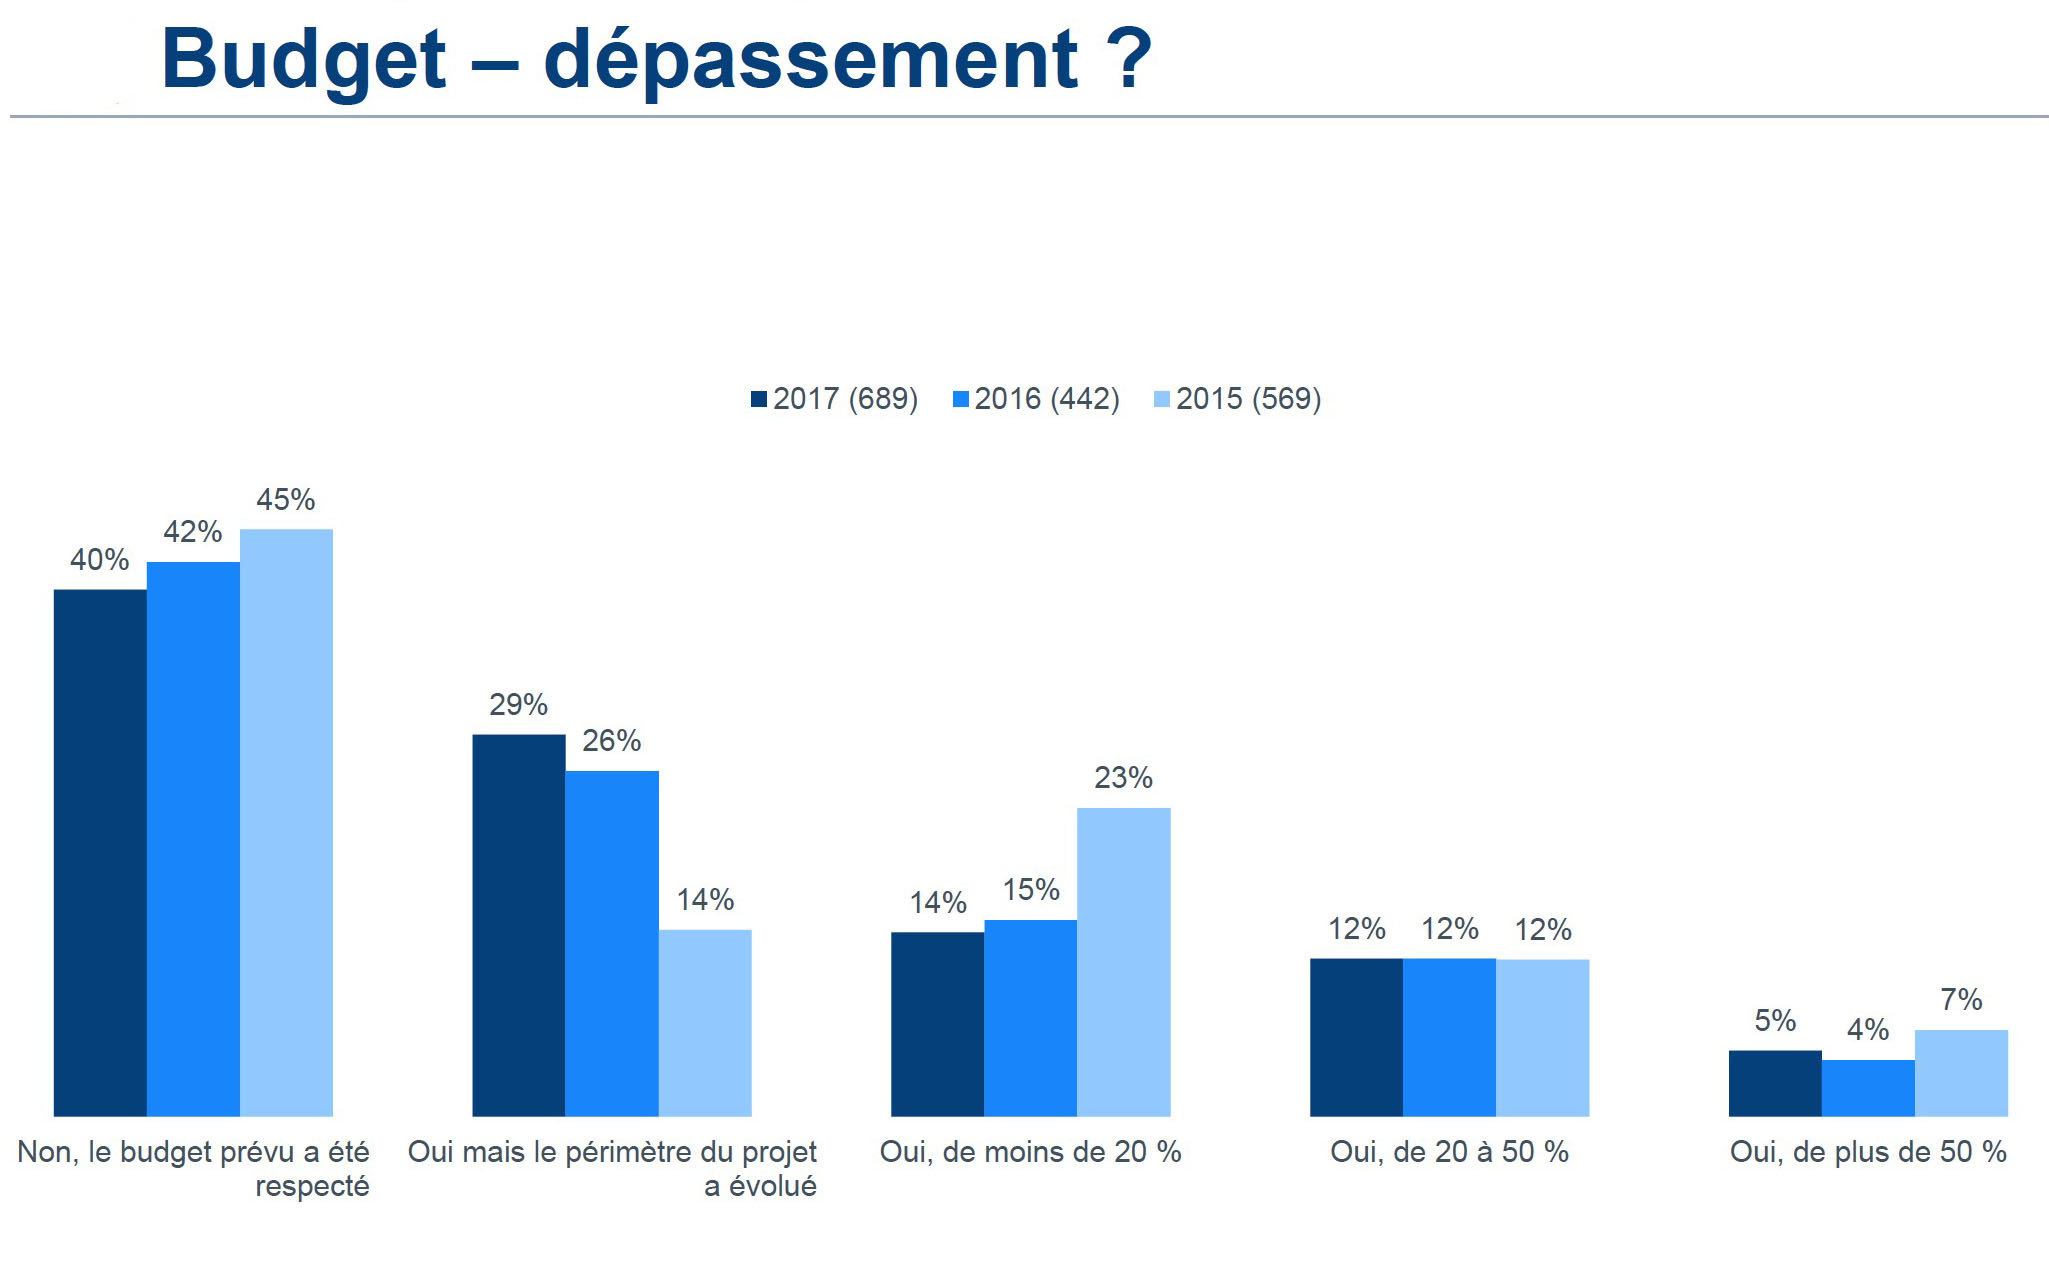
\includegraphics[scale=0.4]{chapitre2/graph-depassement-budget.jpg}
            \caption{Taux du dépassement de budget lors de l’implémentation d’un ERP}
        \end{figure} 

        On peut constater qu’en 2017 plus de 60\% des entreprises qui ont implémenté un ERP ont dépassé le budget prévu, 58\% en 2016 et 55\% en 2015.\\

        En outre du coût, un projet de cette envergure requiert un temps et des ressources qui peuvent dépasser les prévisions, tel que le montre l’étude ERP Report 2010 du cabinet de conseil Panorama Consulting.\\

        \begin{figure}[H]
            \centering
                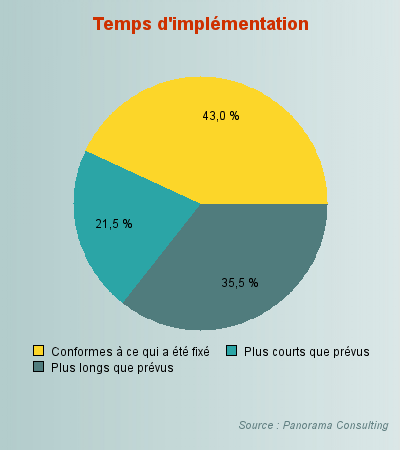
\includegraphics[scale=0.65]{chapitre2/graph-taux-implementation.png}
            \caption{Taux des dépassements des délais lors de l’implémentation d’un ERP}
        \end{figure} 

        Cette étude montre que plus de 35.5\% des entreprises ayant mis en place un ERP, ont vu le temps prévu pour l’implémentation dépassée, il est aussi à noter que la durée moyenne de la mise en place d’un ERP est de 18,4 mois qui varient d’un éditeur à un autre.

    \subsection{Fonctionnalités}
        L’ERP gère et organise les informations de l’ensemble des services de l’entreprise de façon automatique et dynamique, de l’achat des ressources à la vente en passant par la production, ces fonctionnalités sont nombreuses. Les modules plus couramment utilisés sont les suivants : \\
        
        \begin{itemize}
            \item Gestion d’achats
            \item Gestion de la chaine logistique
            \item Gestion de stock et d’inventaire
            \item Gestion de production
            \item Gestion de projet
            \item Gestion des ressources humaines 
            \item Gestion comptabilité
            \item Gestion commerciale
            \item CRM : Gestion des relations clients\\
        \end{itemize}

        Chaque module couvre des fonctionnalités qui lui sont propres, dans le tableau ci-dessous une présentation de certains modules et des fonctionnalités qu’ils proposent.

        \begin{table}[H]
        \begin{center}

        \begin{tabular}{|F{4cm}|R{10cm}|}
        \hline
        \textbf{Modules}  & \makecell[c]{\textbf{Fonctionnalités}} \\
        \hline
        Achats
        &
        Gestion de toutes les transactions comptables, telle que les bons de commande pour l’approvisionnement. Etc.\\

        \hline
        Chaine logistique
        &
        Gestion des ressources utilisées pour le pilotage de la chained’approvisionnement et de livraison.\\

        \hline
        Stock
        &
        Gestion des mouvements du stock, état du stock, entreposage.\\

        \hline
        Production
        &
        La gestion de la production, permet de réguler l’offre et les besoins en
        ressources par apport à la demande, impliquent la planification des ordres
        de fabrication et le contrôle de qualité.\\
        
        \hline
        Gestion de projet
        &
        Gestion de l’ensemble des projets de l’entreprise, de ces tâches et de ces plannings.\\

        \hline
        Ressources humaines
        &
        Gestion des ressources humaines et l’organisation de la rémunération des employés ainsi que des plannings de travail de ceux-ci.\\
        

        \hline
        Comptabilité
        &
        Gestion des obligations comptable auxquelles l’entreprise est soumise et suivie en temps réel de la santé financière de celle-ci, ainsi que de la gestion de facturation et des multidevises.\\

        \hline
        Commerciale
        &
        Gestion de l’aspect commerciale de l’entreprise, permet la gestion de l’ensemble des commandes clients et de leur facturation, permet aussi la réalisation de devis rapide et précise.\\

        \hline
        CRM
        &
        Gestion des relations clients, permet de réaliser de meilleurs suivis de
        l’environnement : clients, fournisseurs, prospects. etc.\\
 
        
        \hline
        \end{tabular}	
        \caption{Les Modules d'un ERP et leurs fonctionnalités}
            \end{center}
        \end{table}	

    \subsection{Conclusion}
        Après avoir défini lors de la première partie le concept d’entreprise, l’environnement et les contraintes auxquelles elle fait face. L’obligation de dégager un bénéfice est vitale, mais un certain nombre de points complexifient leurs systèmes d’information et freine la croissance économique de celle-ci, ces mêmes points qui rendent le recours à une technologie de l’information telle que l’ERP presque obligatoire.\\

        Dans le deuxième point nous avons étudié l’ERP qui est au cœur du système d’information et qui permet la gestion de tous les services de l’entreprise. Ainsi que les avantages et les inconvénients à recourir à un tel outil.\\

        Ensuite nous allons approfondir la recherche et étudier lors du deuxième chapitre, la gestion de stocks et d’approvisionnement.


\newpage

\leftskip=0cm
\renewcommand{\bibname}{Référence bibliographique et webographique du chapitre 2}
\bibliographystyle{ieeetr}	
\bibliography{chapitre2/chap2}